% !Mode:: "TeX:UTF-8"
% !TEX program  = xelatex
\documentclass[a4paper]{article}
\usepackage{amsmath}
\usepackage{amssymb}
\usepackage{ctex}
%\usepackage{braket}
\usepackage[european]{circuitikz}
\usepackage{multirow}
\usepackage{float}
\usepackage{geometry}
\geometry{left=2.5cm,right=2.5cm,bottom=2.5cm,top=2.5cm}
\title{模电实验报告4:差动放大电路实验}
\author{xy\quad 学号\quad 匡亚明学院}
\date{2019年2月29日}
\begin{document}
\maketitle
\bibliographystyle{unsrt}
%--------main-body------------

\section{实验目的}
\begin{enumerate}
\item 进一步熟悉差动放大器的工作原理
\item 掌握测量差动放大器性能的方法
\end{enumerate}

\section{实验仪器}
双踪示波器、信号发生器、交流毫伏表、数字万用表。

\section{预习内容}
\begin{enumerate}
\item 差动放大器的工作原理性能
\item 根据图(\ref{cd})画出单端输入、双端输出的差动放大器的交流微变等效电路图
\end{enumerate}

\section{实验内容}
实验电路如图(\ref{cd})。它是一个具有恒流源的差动放大电路。在输入端,幅值大小相等,相位相反的信号称为差模信号;幅值大小相等,相位相同的干扰称为共模干扰。差动放大器由两个对称的基本共射放大电路组成,发射极负载是一晶体管恒流源。若电路完全对称,对于差模信号, 若$Q_1$的集电极电流增加, 则$Q_2$的集电极电流一定减少,增加与减少之和为零,$Q_3$和$R_{e3}$等效于短路,$Q_1$、$Q_2$的发射极等效于无负载,差模信号被放大。对于共模信号, 若$Q_1$的集电极电流增加, 则$Q_2$的集电极电流一定增加,两者增加的量相等,$Q_1$、$Q_2$的发射极等效于分别接了两倍的恒流源等效电阻,强发射极负反馈使共射放大器对共模干扰起强衰减作用,共模信号被衰减。从而使差动放大器有较强的抑制共模干扰的能力。调零电位器$R_p$用来调节$T_1$、$T_2$管的静态工作点,希望输入信号$V_i$=0时,使双端输出电压$V_o$=0。
\begin{figure}[!h]
\centering
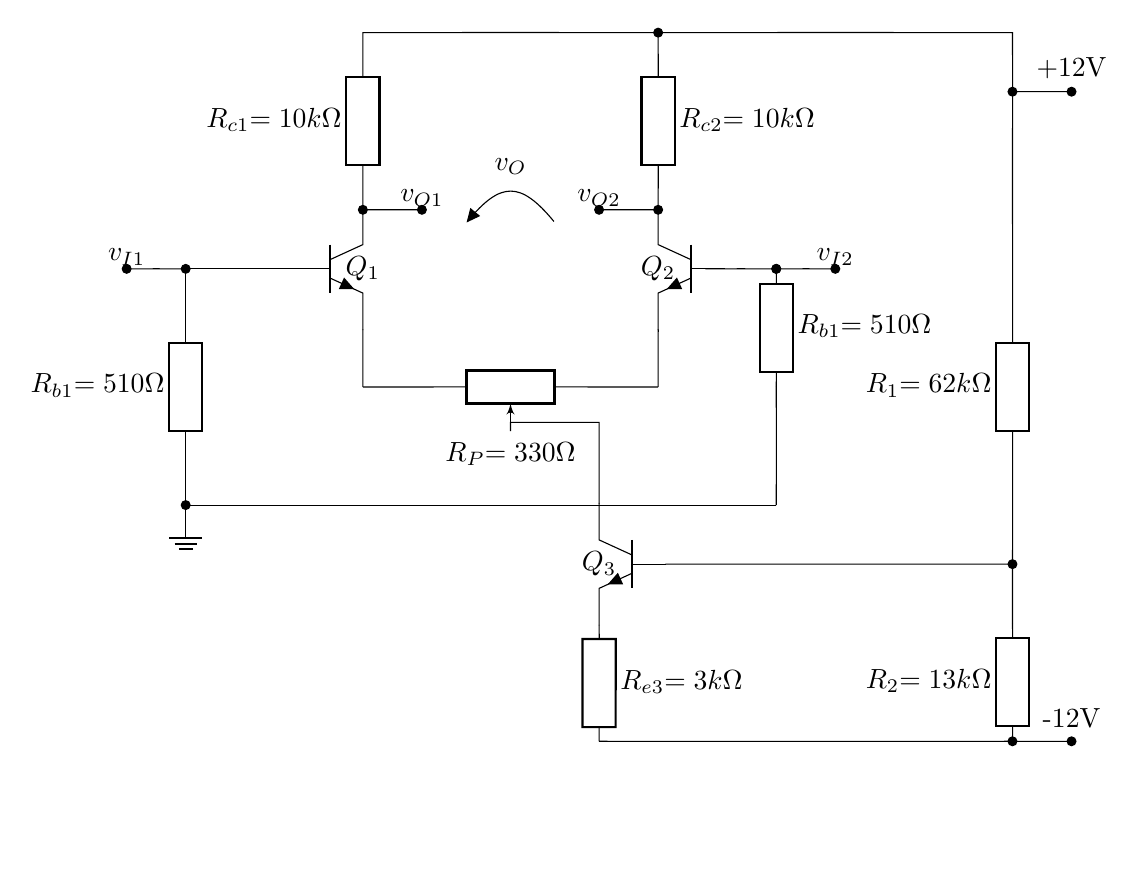
\begin{tikzpicture}[scale=1.5]
\draw (0,0) to [short, *-] (5,0);
\draw (5,0) to [short] (5,1);
\draw (5,1) to [R, l_ = $R_{b1}{=510}\Omega$, -*] (5,2);
\draw (5,2) to [short, *-*] (5.5,2);
\draw (5,2) to [short] (4.4,2);
\draw [anchor=east] (4,2) node[npn, xscale = -1](Q2){};
\draw (Q2.E) to (4,1);
\draw (Q2.C) to (4,2.5) to [short,*-*] (3.5,2.5);

\draw (4,1) to [pR, l = $R_P{=330}\Omega$, n = RP] (1.5,1);
\draw (0,0) to [R, l = $R_{b1}{=510}\Omega$, -*] (0,2);
\draw (0,2) to [short, -*] (-0.5, 2);
\draw (0,2) to (1.1,2);
\draw (1.5,2) node[npn](Q1){};
\draw (Q1.E) to (1.5,1);
\draw (Q1.C) to (1.5,2.5) to [short,*-*] (2,2.5);
\draw (1.5,2.5) to [R,l = $R_{c1}{=10k}\Omega$] (1.5,4) to [short] (4,4) to [R,l = $R_{c2}{=10k}\Omega$] (4,2.5);
\draw (4,4) to [short,*-] (7,4) to [short] (7,3) to [R,l_ = $R_1{=62k}\Omega$] (7,-1);
\draw (7,-1) to [R,l_ = $R_2{=13k}\Omega$] (7,-2);
\draw (7,-3) [short, *-*] (7.5,-3);
\draw (3.5,-0.5) node[npn, xscale = -1](Q3){};
\draw (Q3.B) to [short, -*] (7,-0.5);
\draw (Q3.E) to [R,l = $R_{e3}{=3k}\Omega$] (3.5,-2);
\draw (Q3.C) to (3.5, 0.7) to (2.75,0.7) to (RP.wiper);
\draw (3.5,-2) to [short] (7,-2);
\draw (7,-2) to [short, *-*] (7.5,-2);
\draw (7,3.5) to [short,*-*] (7.5,3.5);

\draw (3.3,2.4) to [open, v=$v_O$] (2.2,2.4);

\draw (0,0) node[ground](GND){};

\draw
{(-0.5,2.1) node{$v_{I1}$}}
{(1.5,2) node{$Q_1$}}
{(4,2) node{$Q_2$}}
{(3.5,-0.5) node{$Q_3$}}
{(5.5,2.1) node{$v_{I2}$}}
{(2,2.6) node{$v_{O1}$}}
{(3.5,2.6) node{$v_{O2}$}}
{(7.5,3.7) node{+12V}}
{(7.5,-1.8) node{-12V}}
;
\end{tikzpicture}
\caption{差动放大电路}\label{cd}
\end{figure}

差动放大器常被用做前置放大器。前置放大器的信号源往往是高内阻电压源,这就要求前置放大器有高输入电阻,这样才能接收到信号。有的共模干扰也是高内阻电压源,例如在使用50Hz工频电源的地方,50Hz工频干扰源就是高内阻电压源。若放大器的输入电阻很高,放大器在接收信号的同时,也接收到了共模干扰。于是人们希望只放大差模信号、不放大共模干扰的放大器,这就是差动放大器。运算放大器的输入级大都为差动放大器,输入电阻都很大,例如,LF353的输入电阻约为$10^{12}$$\Omega$量级,OP07的输入电阻约为$10^7$$\Omega$量级。

本实验电路在两个输入端分别接了510$\Omega$电阻,使差动放大器的输入电阻下降至略小于510$\Omega$,这是很小的输入电阻。其原因是,本实验电路用分列元件组成,电路中对称元件的数值并不完全相等;其集电极为电阻负载,而不是恒流源负载;其发射极为恒流源负载,而不是镜像电流源负载,所以本实验电路的共模抑制比并不高。若本实验电路在输入端不接510$\Omega$电阻,其输入电阻将较大,而共模抑制比不够高,实验环境中存在的高内阻共模干扰将进入输入端,那么输出端的共模干扰将较大,以致使验证差动放大器特性的实验难以进行。由于实验中所用信号源都为低输出电阻信号源,所以输入端接上510$\Omega$电阻后几乎不影响实验电路接收来自信号源的信号,而高内阻共模干扰因实验电路输入电阻大大下降而基本上被拒之输入端外,从而使得输出端的共模干扰很小,实验得以顺利进行。输入端接510$\Omega$电阻并不该变差动放大器的共模抑制比。

由此可见,降低差动放大器输入电阻,可提高差动放大器的抗高内阻共模干扰的能力。

实验者若得到教师的同意,可去掉实验电路中的两个510$\Omega$电阻,再做实验就会发现,实验电路输出端的共模干扰明显增加。
\begin{enumerate}
\item 静态工作点调整与测量\\
将两个输入端$V_{i1}$、$V_{i2}$接地,调整电位器$R_p$使$V_{C1} = V_{C2}$,测量并填写表(\ref{Q})。由于元件参数的离散,有的实验电路有可能最终只能调到$V_{C1} \approx V_{C2}$。静态调整得越对称,该差动放大器的共模抑制比就越高。\\
在测量中应注意两点。一是所有的电压值都应是对“地”测量值。二是应使测量的值有三位以上的有效数字。若用FLUKE45台式数字万用表测量,应选择“SLOW READING RATE”,这时它显示5个测量数字,有效数字为四个。若用普通三位半数字万用表表测量,它最多显示四个数字,其中有效数字为三个,在测量过程中应选择量程,例如,测$V_{C1}$应选“20V”档,测$V_{E1}$应选“2V”档。
%----------table 1--------------------
\item 测量双端输入差模电压放大倍数\\
在实验箱上调整DC信号源,使OUT1大约为0.1V、OUT2大约为-0.1V,然后分别接至$V_{i1}$、$V_{i2}$,再调整,使OUT1为0.1V、OUT2为-0.1V,测量、计算并填写表(\ref{AD2table})。
%----------table 2--------------------
这样做的原因是,实验电路的输入端对“地”接有510$\Omega$电阻,实验箱上的可变直流电压源是用1k$\Omega$可变电阻对5V、0.5V直流电压分压实现的,即直流电压信号源内阻与实验电路输入电阻大小可比。直流电压信号源接负载时的电压将明显小于未接负载时的电压,所以必须将直流电压信号源与实验电路连接后,再把输入电压调到所需要的电压值。\\
这里,双端输入差模电压单端输出的差模放大倍数应用下式计算:
\begin{equation}
A_{D1} = \cfrac{v_{C1}-V_{C1}}{v_{\text{ID}}}\label{AD1}
\end{equation}
\item 测量双端输入共模抑制比CMRR\\
将两个输入端接在一起,然后依次与OUT1、OUT2相连,记共模输入为$V_{iC}$。测量、计算并填写表(\ref{CMRRtable})。若电路完全对称,则$v_{C1}$-$v_{C2}$=$v_o$=0,实验电路一般并不完全对称,若测量值有四位有效数字,则$v_o$不应等于零。
这里,双端输入共模电压单端输出的共模放大倍数应用下式计算:
\begin{equation}
A_{C1} = \cfrac{v_{C1}-V_{C1}}{c_{IC}}
\end{equation}
建议CMRR用dB表示
%-----table 3----------------------------
\begin{equation}
\text{CMRR} = 20\text{lg}\left|\frac{A_D}{A_C}\right|\text{dB}
\end{equation}
\item 测量单端输入差模电压放大倍数\\
将$V_{i2}$接地,$V_{i1}$依次与OUT1、OUT2相连,然后再接入f=1KHz、有效值为50mV的正弦信号,测量、计算并填写表(\ref{AD1table})。若输入正弦信号,在输出端,$v_{C1}$、$v_{C2}$的相位相反,所以双端输出$v_o$的模是$v_{C1}$、$v_{C2}$的模的和,而不是差。
%-----------table 4---------------------
\end{enumerate}

\section{实验数据}
\begin{enumerate}
\item 调整静态\\
其中$V_{B1}$和$V_{B2}$两项测量值极小,为微安量级,加上电路图中两点接地,因此将其视为0。
\begin{table}[!h]
\centering
\caption{静态工作点}
\label{Q}
\begin{tabular}{|c|c|c|c|c|c|c|c|c|c|}
\hline
对地电压 & $V_{B1}$ & $V_{B2}$ & $V_{B3}$ & $V_{C1}$ & $V_{C2}$ & $V_{C3}$  & $V_{E1}$ & $V_{E2}$ & $V_{E3}$ \\ \hline
测量值(V)  & 0        & 0        & -7.9133 & 6.40173 & 6.40143 & -0.76117 & -0.620     & -0.620  & -8.55716   \\ \hline
\end{tabular}
\end{table}
\item 双端输入差模电压放大倍数\\
式(\ref{AD1})中的$v_{\text{ID}}$ = OUT1 - OUT2.
\begin{table}[!h]
\centering
\caption{双端输入差模电压放大倍数}
\label{AD2table}
\begin{tabular}{|c|c|c|c|c|c|c|c|}
\hline
\multicolumn{5}{|c|}{测量值(V)}                       & \multicolumn{3}{c|}{计算值}      \\ \hline
OUT1    & OUT2     & $v_{C1}$ & $v_{C2}$ & $v_{O}$ & $A_{D1}$ & $A_{D2}$ & $A_D$   \\ \hline
0.10044 & -0.10034 & 3.0882   & 9.7136   & 6.6254  & -16.503  & -16.4965 & 32.9983 \\ \hline
\end{tabular}
\end{table}
\item 双端输入共模抑制比CMRR\\
\begin{table}[!h]
\centering
\caption{测量双端输入共模抑制比CMRR}
\label{CMRRtable}
\begin{tabular}{|c|c|c|c|c|c|c|c|}
\hline
\multirow{2}{*}{输入(V)} & \multicolumn{3}{c|}{测量值(V)}   & \multicolumn{4}{c|}{计算值}                 \\ \cline{2-8} 
                       & $v_{C1}$ & $v_{C2}$ & $v_{O}$ & $A_{C1}$ & $A_{C2}$ & $A_C$    & CMRR    \\ \hline
+0.10056               & 6.3763   & 6.4263   & 0.05    & -0.25289 & 0.2473   & 0.4972   & 36.4389 \\ \hline
-0.10134               & 6.3774   & 6.4261   & 0.0487  & 0.2401   & -0.2434  & -0.48056 & 36.7350 \\ \hline
\end{tabular}
\end{table}
\item 单端输入差模放大倍数\\
\begin{table}[!h]
\centering
\caption{单端输入差模放大倍数}
\label{AD1table}
\begin{tabular}{|c|c|c|c|c|}
\hline
\multirow{2}{*}{输入(V)} & \multicolumn{3}{c|}{测量值(V)}   & \multirow{2}{*}{单端输入放大倍数$A_D$} \\ \cline{2-4}
                       & $v_{C1}$ & $v_{C2}$ & $v_{O}$ &                                \\ \hline
直流+0.10020             & 4.7044   & 8.0965   & 3.3921  & 33.8533                        \\ \hline
直流-0.10145               & 8.0666   & 4.7357   & -3.3309 & 32.8329                        \\ \hline
正弦信号$v_{s}$=0.04523    & 0.7483   & 0.74803  & 1.49633 & 33.0827                        \\ \hline
\end{tabular}
\end{table}
\end{enumerate}

\section{误差分析}
\begin{enumerate}
\item 调整静态\\
实验要求调整静态工作点时使电路完全对称,实际上,即使在某一时刻将$V_{C1}$和$V_{C2}$调至相等,由于仪器的不稳定性,静态工作点也会渐渐发生偏移。在后续实验时,很可能已经偏离静态工作点相当程度,因此产生影响。
\item 电源\\
实验要求电源为恒流源,实际使用的是恒压源,随着电路使用时间的增长,一些元器件(如电阻)因为发热而该改变阻值从而影响电路电流的稳定性,造成影响。
\item 零点漂移$^{\cite{jiaocai}}$\\
零点漂移指当放大电路的输入端短路时,输出端还有缓慢变化的电压产生的现象。这种现象的主要原因是温度引起的半导体元件参数变化。尽管差动放大器可以抑制零点漂移,但是若电路不完全对称,则还可能会有零点漂移的现象。
\end{enumerate}

\section{思考题}
\begin{enumerate}
\item \textbf{实验箱上的双端输入差动放大器的共模抑制比不算高,若要进一步提高共模抑制比,可采取哪些办法?}\\
\begin{enumerate}
\item 从前文可知,如果电路完全对称,则CMRR理论上应为无穷大。所以尽可能的把电路调整对称有助于增大CMRR。
\item 从教材$^{\cite{jiaocai}}$7.2节相关内容可知:
$$\text{CMRR} \approx \cfrac{\beta r_o}{r_{be}}$$
其中$r_o$为理想情况下滑动变阻器接入电路的阻值相等的两部分的阻值。因此提高滑动变阻器$R_P$的阻值可以增大CMRR。
\item 由上一点的公式,选用$\beta$值较大的三极管也可以增大CMRR。
\end{enumerate}
\item \textbf{图(1)中的电阻$R_{b1}$、$R_{b2}$在电路中起什么作用?若去掉$R_{b1}$、$R_{b2}$,按本实验(3)的方法和步骤再测CMRR,两次测量的结果是否会有较大差别?为什么?}\\
作用:使得放大器的输入电阻略微小于510$\Omega$,这是个很小的输入电阻,可以提高放大器抗高内阻共模干扰的能力。\\
若去掉,测量过程中的电压数值可能会有变化,但不会影响CMRR。去掉这两个电阻,会使输入电阻较大,实验环境存在的高内阻共模干扰将进入输入端,使输出端的共模干扰较大,以致实验难以进行,测得数据也应该发生变化。CMRR不变是书中给出的。
\item \textbf{归纳差动放大器的特点与性能,并与共射放大器比较。}\\
差动放大器用双倍的元器件换来对共模干扰的抑制,使得放大器性能更加稳定,但是放大倍数明显比共射放大器小。如前文误差分析提到,若电路对称性较好,差动放大器可以很好的抑制零点漂移,这是共射放大器难以实现的。
\end{enumerate}
%--------bib------------------
\bibliography{ref}
\end{document}